\begin{proof}
Recall that in the backbone notation $n$ denotes the total number of parties,
$t$ denotes the number of adversarial parties, $q$ denotes the number of the
random oracle queries allowed per party per round and $p$ is the probability that
one random oracle query will be successful and remember that $p = T / 2^\kappa$
where $T$ is the mining target and $\kappa$ is the security parameter (or hash
function bit count). Then $f$ denotes the probability that a given round is
successful and we have that $f = 1 - (1 - p)^{q(n-t)}$. Recall further that a
requirement of the backbone protocol is that the honest majority assumption is
satisfied, that is that $t \leq (1 - \delta)(n - t)$ were $\delta \geq 2f +
3\epsilon$, where $\epsilon \in (0, 1)$ is an arbitrary small constant describing
the quality of the concentration of the random variables.

Denote $\alpha_\mathcal{A}$ the secret chain generated by the adversary and
$\alpha_B$ the honest chain belonging to any honest party. We will show that
for certain protocol values we have that
$\Pr[|\alpha_\mathcal{A}\upchain^\mu| \geq |\alpha_B\upchain^\mu|]$ is
overwhelming.

Assume that, to the adversary's harm and to simplify the analysis, the adversary
plays at beginning of every round and does not perform adversarial scheduling.
At the beginning of the round when it is the adversary's turn to play, she has
access to the blocks diffused during the previous round by the honest parties.

First, observe that at the beginning of each round, the adversary finds herself
in one of two different situations: Either she has been forced into an
$r$-round-long period of suppression, or she is not in that period. If she is
within that period, she blindly performs the suppression attack without regard
for the state of the world. If she is not within that period, then she must
initially observe the blocks diffused at the end of the previous round by the
honest parties. Call these rounds during which the diffused data must be
examined by the adversary \textit{decision rounds}. Let there be $\omega$
decision rounds in total. In each such decision round, it is possible that the
adversary discovers a diffused $\mu$-superblock and therefore decides that a
suppression attack must be performed starting with the current round. Call these
rounds during which this discovery is made by the adversary \textit{migration
rounds}. Let there be $y$ migration rounds in total. The adversary devotes the
migration round to performing the suppression attack as well as $r - 1$
non-migration rounds after the migration round. Call these rounds, including the
migration round, \textit{suppression rounds}. In the rest of the decision
rounds, the adversary will not find any $\mu$-superblocks diffused. Call these
\textit{secret chain rounds}; these are rounds where the adversary devotes her
queries to mining on the secret chain. Let there be $x$ secret chain rounds. If
the adversary devotes $\omega$ decision rounds to the attack in total, then
clearly we have that $\omega = x + y$. If the total number of rounds during
which the attack is running is $s$ then we also have that $s = x + ry$, because
for each migration round there are $r - 1$ non-decision rounds that follow.

\begin{figure*}[t]
    \caption{The double spending attack.
    The top chain fork is wholly adversarially mined, while the bottom is
    honestly adopted. Gray blocks are adversarially mined 0-blocks.
    Black blocks are $\mu$-superblocks.}
    \centering
    \iftwocolumn
        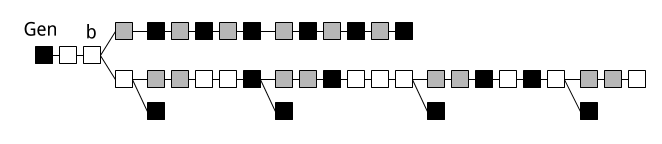
\includegraphics[width=1.5\columnwidth,keepaspectratio]{figures/double-spend-popow.png}
    \else
        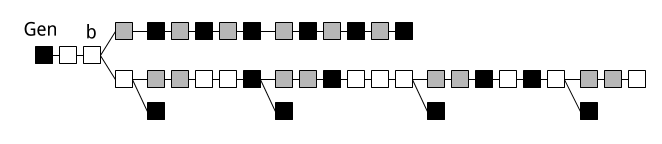
\includegraphics[width=0.7\columnwidth,keepaspectratio]{figures/double-spend-popow.png}
    \fi
    \label{fig.double-spend}
\end{figure*}

We will analyze the honest and adversarial superchain lengths with respect to
$\omega$, which roughly corresponds to time (because note that $\omega \geq
s/r$, and so $\omega$ is proportional to the number of rounds).
Let us calculate the probability $p_{SB}$ (``superblock probability'') that a
decision round ends up being a migration round. Ignoring the negligible event
that there will be random oracle collisions, we have that $p_{SB} = (n -
t)qp2^{-\mu}$.

Given this, note that the decision taken at the beginning of each decision round
follows independent Bernoulli distributions with probability $p_{SB}$. Denote
$z_i$ the indicator random variable indicating whether the decision round was
a migration round. Therefore we can readily calculate the expectations for the
random variables $x$ and $y$, as $x = \omega - y$, $y = \sum_{i=1}^\omega z_i$.
We have $E[x] = (1 - p_{SB})\omega$ and $E[y] = p_{SB}\omega$. Applying a
Chernoff bound to the random variables $x$ and $y$, we observe that they will
attain values close to their mean for large $\omega$ and in particular
$\Pr[y \geq (1 + \delta)E[y]] \leq \exp(-\frac{\delta^2}{3} E[y])$ and similarly
$\Pr[x \leq (1 - \delta)E[x]] \leq \exp(-\frac{\delta^2}{2} E[x])$, which are
negligible in $\omega$.

Given that there will be $x$ secret chain rounds, we observe that the random
variable indicating the length of the secret adversarial superchain follows the
binomial distribution with $xtq$ repetitions and probability $p2^{-\mu}$. We
can now calculate the expected secret chain length as
$E[|\alpha_\mathcal{A}\upchain^\mu|] = xtqp2^{-\mu}$. Observe that in this
probability we have given the adversary the intelligence to continue using her
random oracle queries during a round even after a block has been found during a
round and not to wait for the next round. Applying a Chernoff bound, we obtain
that $\Pr[|\alpha_\mathcal{A}\upchain^\mu| \leq (1 -
\delta)E[|\alpha_\mathcal{A}\upchain^\mu|]] \leq
exp(-\frac{\delta^2}{2}E[|\alpha_\mathcal{A}\upchain^\mu|])$, which is
negligible in $\omega$ (because we know that with overwhelming probability $x >
(1 - \delta)(1 - p_{SB})\omega$).

It remains to calculate the behavior of the honest superchain.
Suppose that a migration round occurs during which at least one superblock $B$
is diffused. We will now calculate the probability $p_{sup}$ that the adversary
is able to suppress that block after $r$ rounds by performing the suppression
attack and cause all honest parties to adopt a chain not containing $B$.

One way for this to occur is if the adversary has generated exactly $2$ shallow
blocks (blocks which are not $\mu$-superblocks) after exactly $r$ rounds and the
honest parties having generated exactly $0$ blocks after exactly $r$ rounds.
This provides a lower bound for the probability, which is sufficient for our
purposes. Call ADV-WIN the event where the adversary has generated exactly $2$
shallow blocks after exactly $r$ rounds since the diffusion of $B$ and call
HON-LOSE the event where the honest parties have generated exactly $0$ blocks
after exactly $r$ rounds since the diffusion of $B$.

The number of blocks generated by the adversary after the diffusion of $B$
follows the binomial distribution with $r$ repetitions and probability $p_{LB}$,
where $p_{LB}$ denotes the probability that the adversary is able to produce a
shallow block (``low block probability'') during a single round. We have that
$p_{LB} = tqp(1 - 2^{-\mu})$. To evaluate $\Pr[\text{ADV-WIN}]$, we evaluate the
binomial distribution for $2$ successes to obtain $\Pr[\text{ADV-WIN}] =
\frac{r(r - 1)}{2} p_{LB}^2 (1 - p_{LB})^{r - 2}$. The number of blocks
generated by the honest parties after the diffusion of $B$ follows the binomial
distribution with $r$ repetitions and probability $f$. To evaluate
$\Pr[\text{HON-LOSE}]$, we evaluate the binomial distribution for $0$ successes
to obtain $\Pr[\text{HON-LOSE}] = (1 - f)^r$. Note that this is an upper bound
in the probability, in particular because there can be multiple
blocks during a non-uniquely successful round during which a $\mu$-superblock
was generated.

Then observe that the two events ADV-WIN and HON-LOSE are independent and
therefore
$p_{sup} =
 \Pr[\text{ADV-WIN}]\Pr[\text{HON-LOSE}] =
 \frac{r(r - 1)}{2} p_{LB}^2 (1 - p_{LB})^{r - 2}(1 - f)^r$.

Now that we have evaluated $p_{sup}$,  we will calculate the honest chain length
in two chunks: The superblocks generated and adopted by the honest parties
during secret chain rounds, $\chain_1$, and the superblocks generated and
adopted by the honest parties during suppression rounds, $\chain_2$ (and note
that these sets of blocks are not blockchains on their own).

$|\chain_1|$ is a random variable following the binomial distribution with
$s(n - t)q$ repetitions and probability $p2^{-\mu}(1 - p_{sup})$. In the
evaluation of this distribution, we give the honest parties the liberty to
belong to a mining pool and share mining information within a round, an
assumption which only makes matters for the adversary worse. We can now
calculate the expected length of $\chain_1$ to find
$E[|\chain_1|] = s(n - t)qp2^{-\mu}(1 - p_{sup})$. Applying a Chernoff bound, we
find that
$\Pr[|\chain_1| \geq (1 + \delta)E[|\chain_1|]]
\leq exp(-\frac{\delta^2}{3}E[|\chain_1|])$, which is negligible in $s$.

Finally, some additional $\mu$-superblocks could have been generated by the
honest parties while the adversary is spending $r$ rounds attempting to suppress
a previous $\mu$-superblock. These $\mu$-superblocks will be adopted in the case
the adversary fails to suppress the previous $\mu$-superblock. As the adversary
does not devote any decision rounds to these new $\mu$-superblocks, they will
never be suppressed if the previous $\mu$-superblock is not suppressed. We
collect these in the set $\chain_2$. To calculate $|\chain_2|$, observe that the
number of unsuppressed $\mu$-superblocks which caused an adversarial suppression
period is $|\chain_1|$. For each of these blocks, the honest parties spend $r$
rounds attempting to form further $\mu$-superblocks on top. The total number of
such attemps is $r|\chain_1|$. Therefore, the number of further honestly
generated $\mu$-superblocks attained during the $|\chain_1|$ different $r$-round
periods follows a binomial distribution with $|\chain_1|rq(n - t)$ repetitions
and probability $p2^{-\mu}$. Here we allow the honest parties to use repeated
queries within a round even after a shallow success and to work in a pool
to obtain an upper bound for the expectation. Therefore $E[|\chain_2|] =
|\chain_1|rq(n - t)p2^{-\mu}$ and applying a Chernoff bound we obtain that
$\Pr[|\chain_2| \geq (1 + \delta)E[|\chain_2|]] \leq
exp(-\frac{\delta}{3}E[|\chain_2|])$, which is negligible in $s$ and has a
quadratic error term. We deduce that $|\chain_2|$ will have a very small length
compared to the rest of the honest chain, as it is a vanishing term in $\mu$.

Concluding the calculation of the adversarial superchain, we get
$E[|\alpha_B\upchain^\mu|] = E[|\chain_1|] + E[|\chain_2|]$.

Finally, it remains to show that there exist values $p, n, t, q, r, \mu, \delta$
such that a $E[|\alpha_\mathcal{A}\upchain^\mu|] \geq (1 +
\delta)E[|\alpha_B\upchain^\mu|]$.
Using the values $p = 10^{-5}, q = 1, n =
1000, t = 489, \mu = 25, r = 200$, we observe that the honest majority
assumption is preserved. Replacing these values into the expectations formulae
above, we obtain $E[|\alpha_\mathcal{A}\upchain^\mu] \approx 1.457 * 10^{-10} *
\omega$ and $E[|\alpha_B\upchain^\mu] \approx 1.424 * 10^{-10} * \omega$, which
result to a constant gap $\delta$. Because the adversarial chain grows linearly
in $\omega$, the adversary only has to wait sufficient rounds for obtaining $m$
blocks to create a valid proof. Therefore, for these values, the adversary
will be able to generate a convincing PoPoW at some level $\mu$ which is longer
than the honest parties' proof, even when the adversary does not have a longer
underlying blockchain.
\Qed
\end{proof}
